The first paper proposed the method LT-FH++, which is an extension of the previously proposed LT-FH method by Hujoel et al\cite{hujoel2020liability}. The notable difference between LT-FH and LT-FH++ is the ability to account for age of onset for cases or age for controls, sex, birth year, as well as the same information in the included family members. The LT-FH method considers parents in the same way and also does not distinguish between the index person and the siblings, regardless of age differences or sex. Another difference is the ability to account for siblings individually rather than considering the number of siblings and an "\textit{at least one affected sibling}" indicator. Considerable changes have also been made to the sampling strategy to allow for the increased flexibility in the family and their thresholds. 

\subsubsection{Simulation results}
We performed simulations to assess the performance of LT-FH++ against LT-FH and a simple linear regression GWAS. The simulations are based on simulated genotypes, where we simulated a pair of parents and one offspring, meaning no siblings. The choice of parameters was heavily inspired by the ones used in the LT-FH paper to ensure compatibility between findings. The simulated genotypes had a heritability on the liability scale of $ h^2 = 0.5 $, a population prevalence of $ 5\% $, with a higher prevalence in one of the simulated sexes. We also considered a population prevalence of $ 10\% $, but they are not shown here. The case ratio was $ 1:4 $ between sexes, and it was also present in the parents. The genotypes consisted of $ 100,000 $ individuals, each with $ 100,000 $ independent SNPs where $ 1000 $ of them were causal, meaning an effect size different from $ 0 $. The simulations shown in Figure \ref{fig:LTFH++_simulation_results} are based on $ 10 $ replications of the genotypes. Case ascertainment is common in biobanks, meaning a higher or lower prevalence of a phenotype of interest compared to the rest of the population. We emulated case ascertainment in the simulations by downsampling the entire population until it had a subpopulation with $ 10,000 $ individuals with a ratio of cases and control of $ 1:1 $.
\begin{figure}[h]
	\label{fig:LTFH++_simulation_results}
	\caption{Simulation results}
	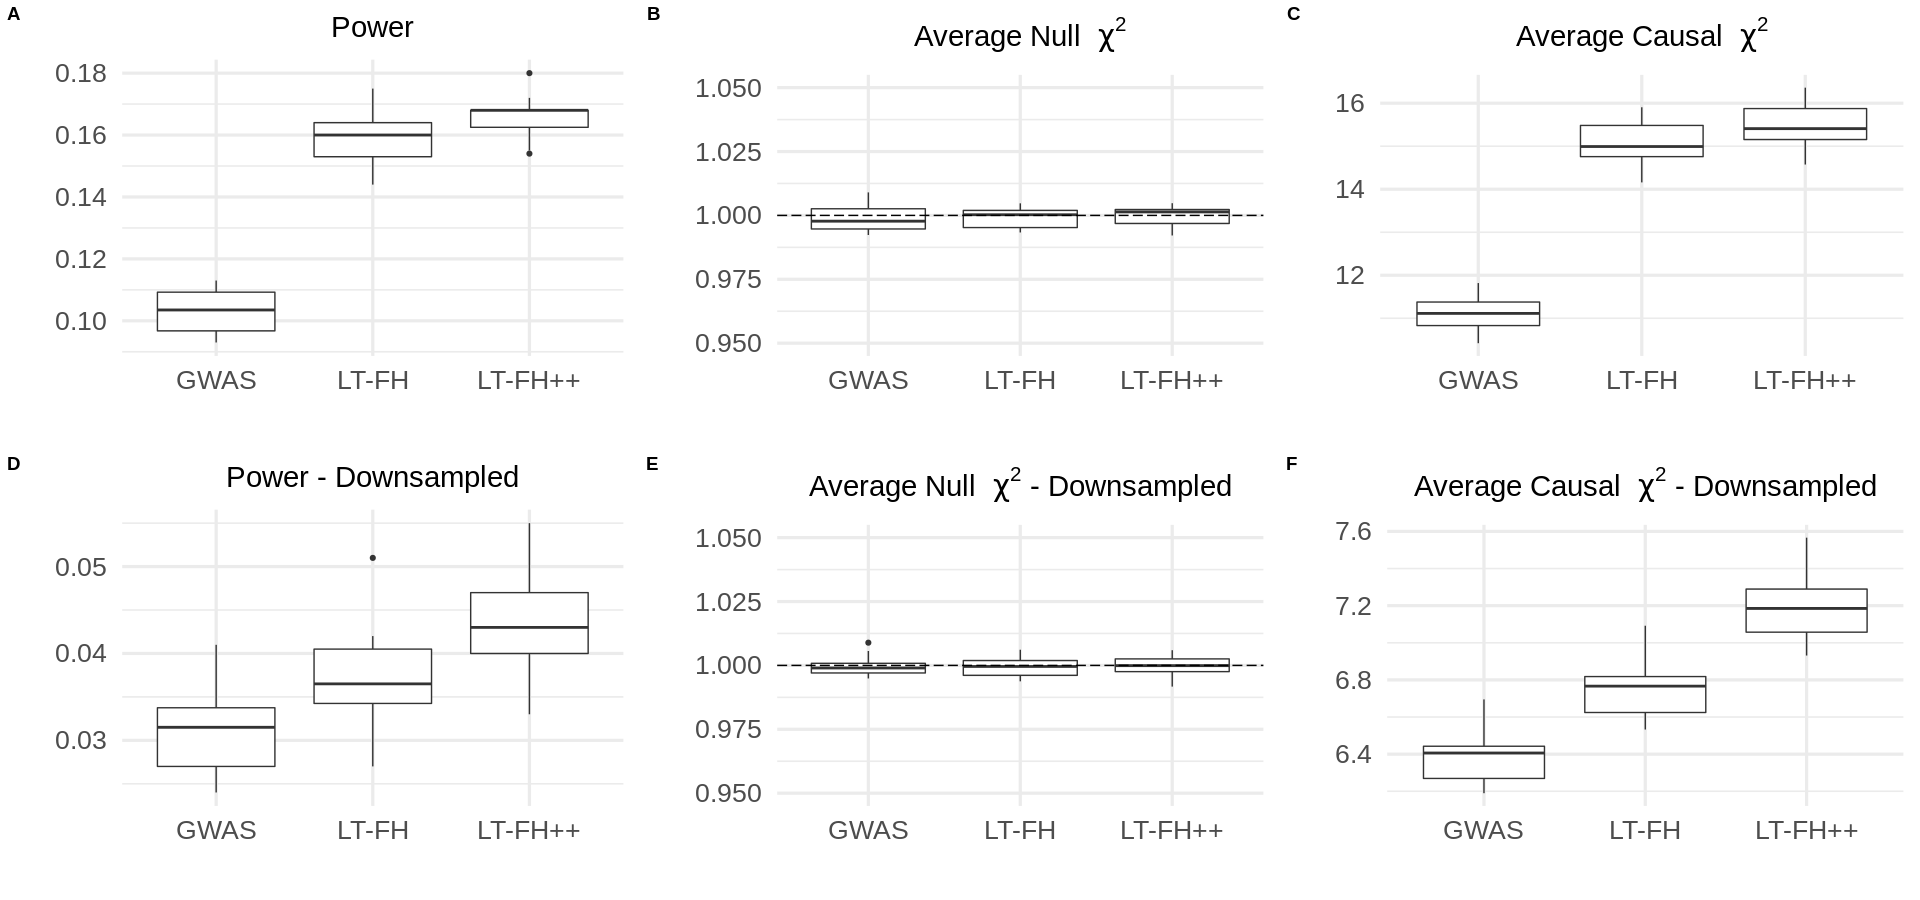
\includegraphics[width=\textwidth]{results/boxplot_05prev_both.pdf}
\end{figure}

The simulations show a modest increase in favour of LT-FH++ over LT-FH in the full sample, with an average power increase across the $ 10 $ simulations of $ 4\% $. Both LT-FH and LT-FH++ has an average power increase of more than $ 50\% $ compared to the case-control status used in \texttt{GWAS}. However, case ascertainment has a significant impact on the ratio between LT-FH and LT-FH++. When case ascertainment is present, the average power increase of LT-FH++ over LT-FH was $ 18\% $.

\subsubsection{Real-world analysis}
LT-FH++ was also applied to four of the focus disorders of iPSYCH and mortality in UKBB. The mortality GWAS in UKBB resulted in $ 0 $ genome-wide significant SNP for simple linear regression, $ 2 $ for LT-FH, and $ 10 $ for LT-FH++. The Manhattan plot for mortality can be found in Figure \ref{fig:LTFH++_manhattanMortality}.
\begin{wrapfigure}{R}{10cm}
	\label{fig:LTFH++_manhattanMortality}
	\caption{Mortality in UKBB}
	%	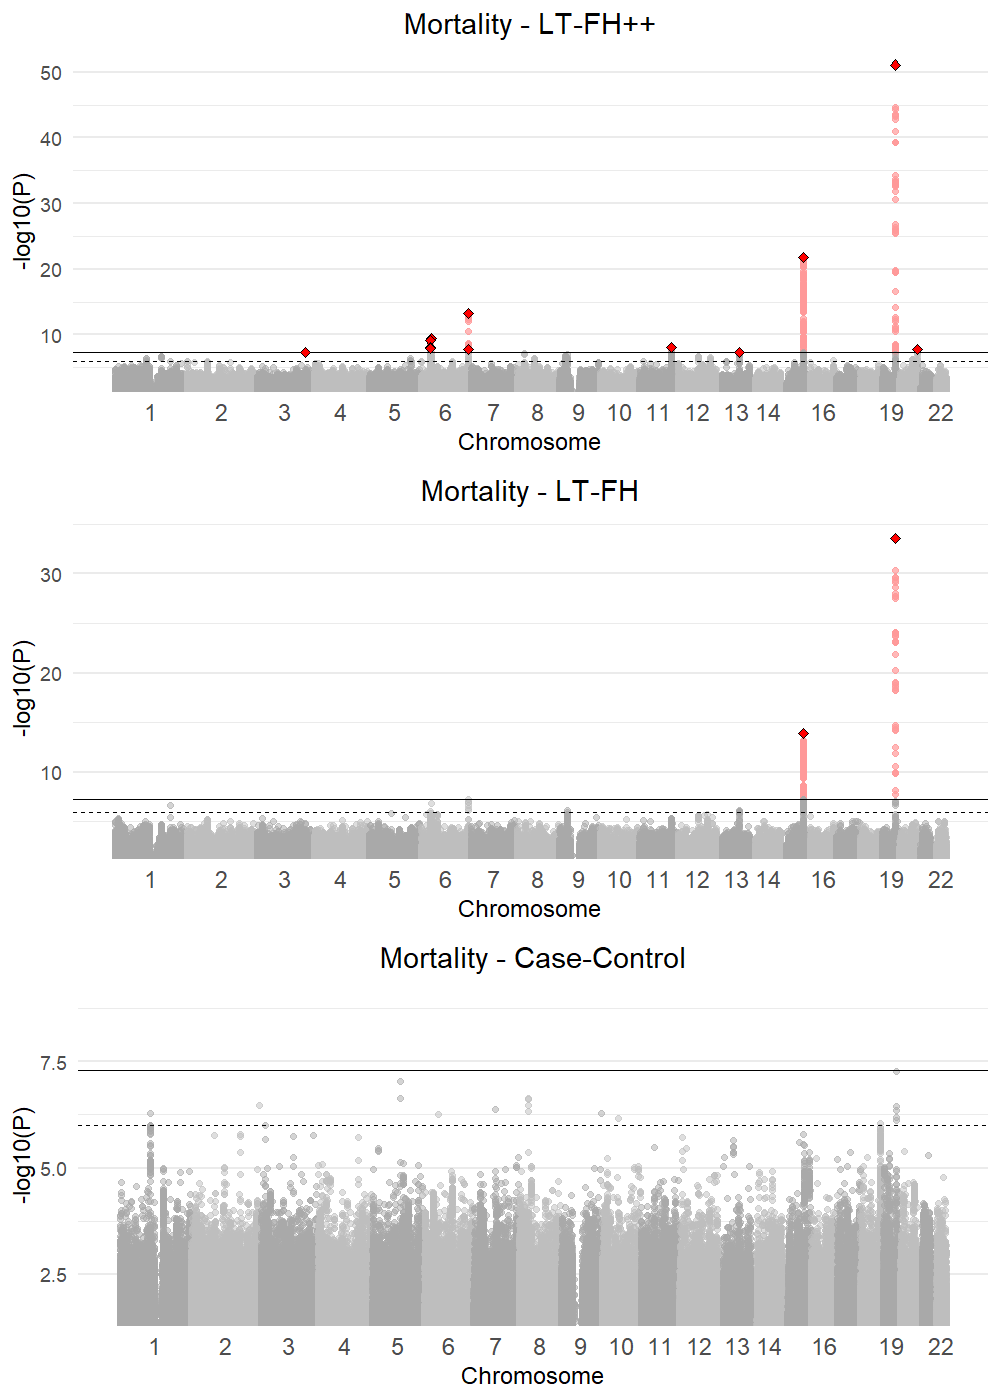
\includegraphics[width=0.7\textwidth]{results/manhattanPlot_mortality.pdf} % adds a lot of loading 
	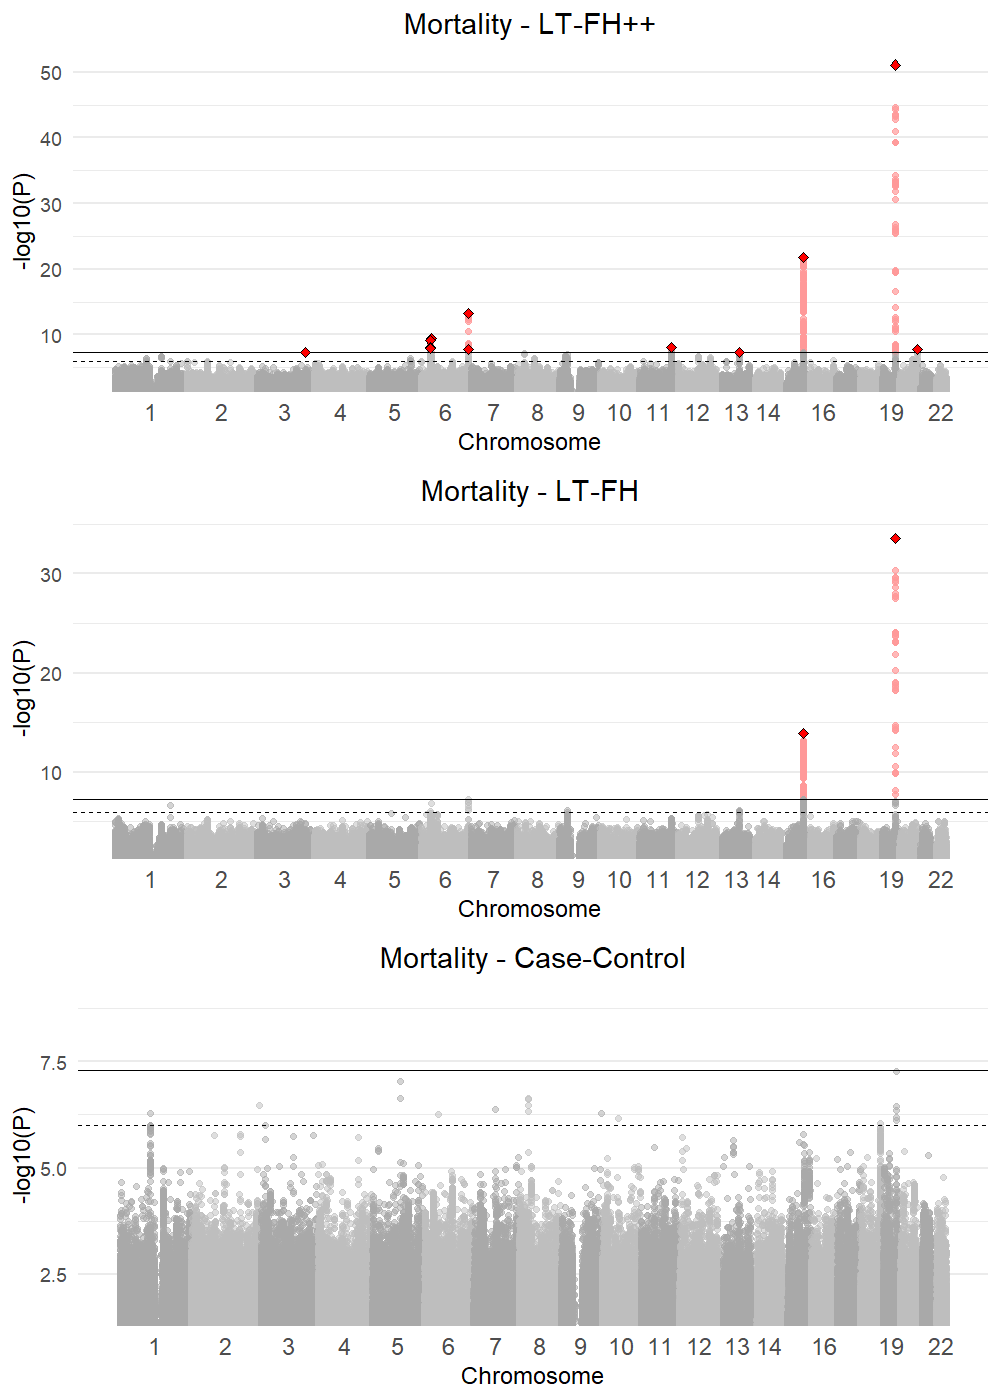
\includegraphics[width=10cm]{results/manhattanPlot_mortality.png}
\end{wrapfigure}
The GWAS performed in iPSYCH did not provide nearly as large of an increase in power for LT-FH++ or LT-FH over simple linear regression. In fact, we did not see any notable improvement over simple linear regression of the case-control status. The Manhattan plot for ADHD in iPSYCH can be found in Figure \ref{fig:LTFH++_manhattanADHD}. We did find $ 7 $ genome-wide significant SNPs for ADHD using LT-FH++ and $ 5 $ for LT-FH and case-control status, but the two additional associations for LT-FH++ were very close to genome-wide significance for the other two outcomes as well.
\begin{wrapfigure}{R}{10cm}
	\label{fig:LTFH++_manhattanADHD}
	\caption{ADHD in iPSYCH}
	%	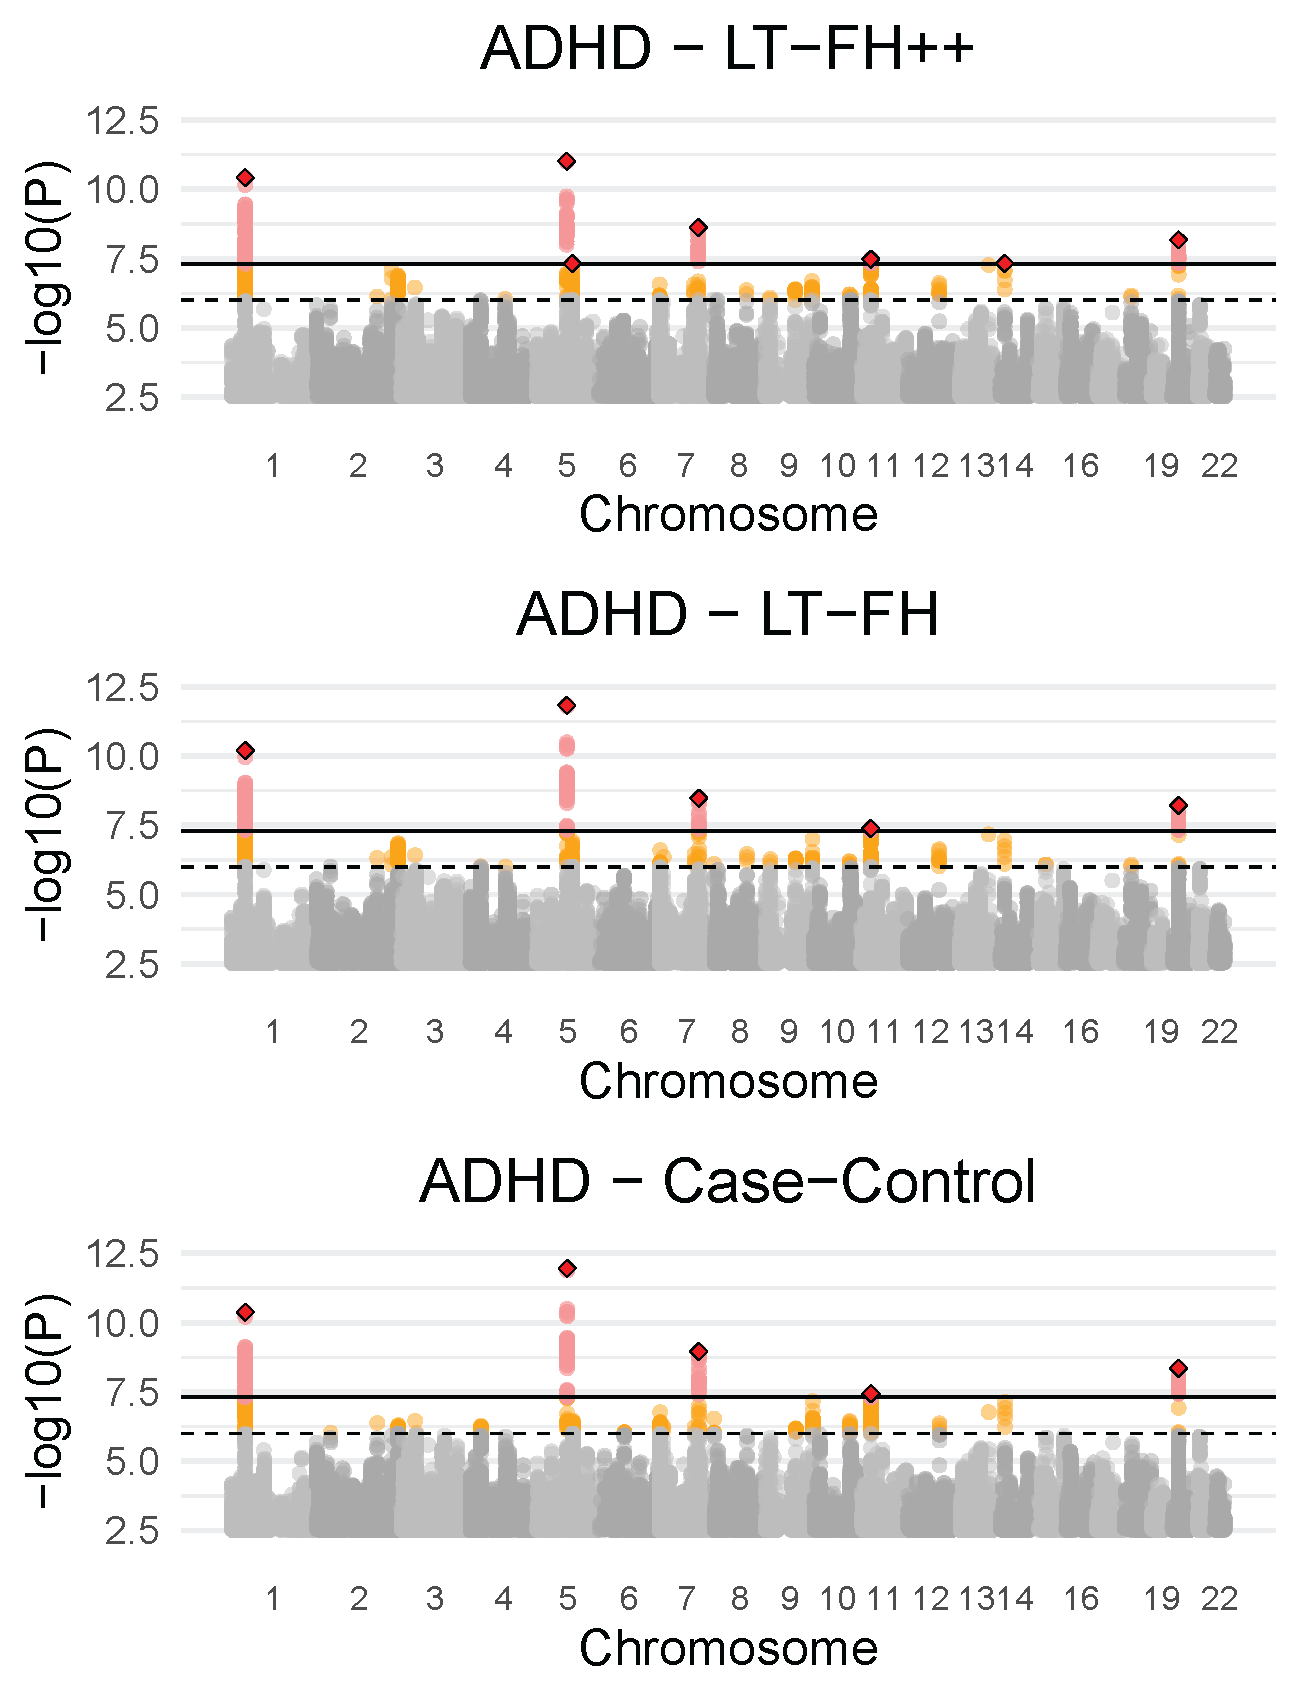
\includegraphics[width=0.7\textwidth]{results/manhattanPlot_ADHD.pdf} % adds a lot of loading 
	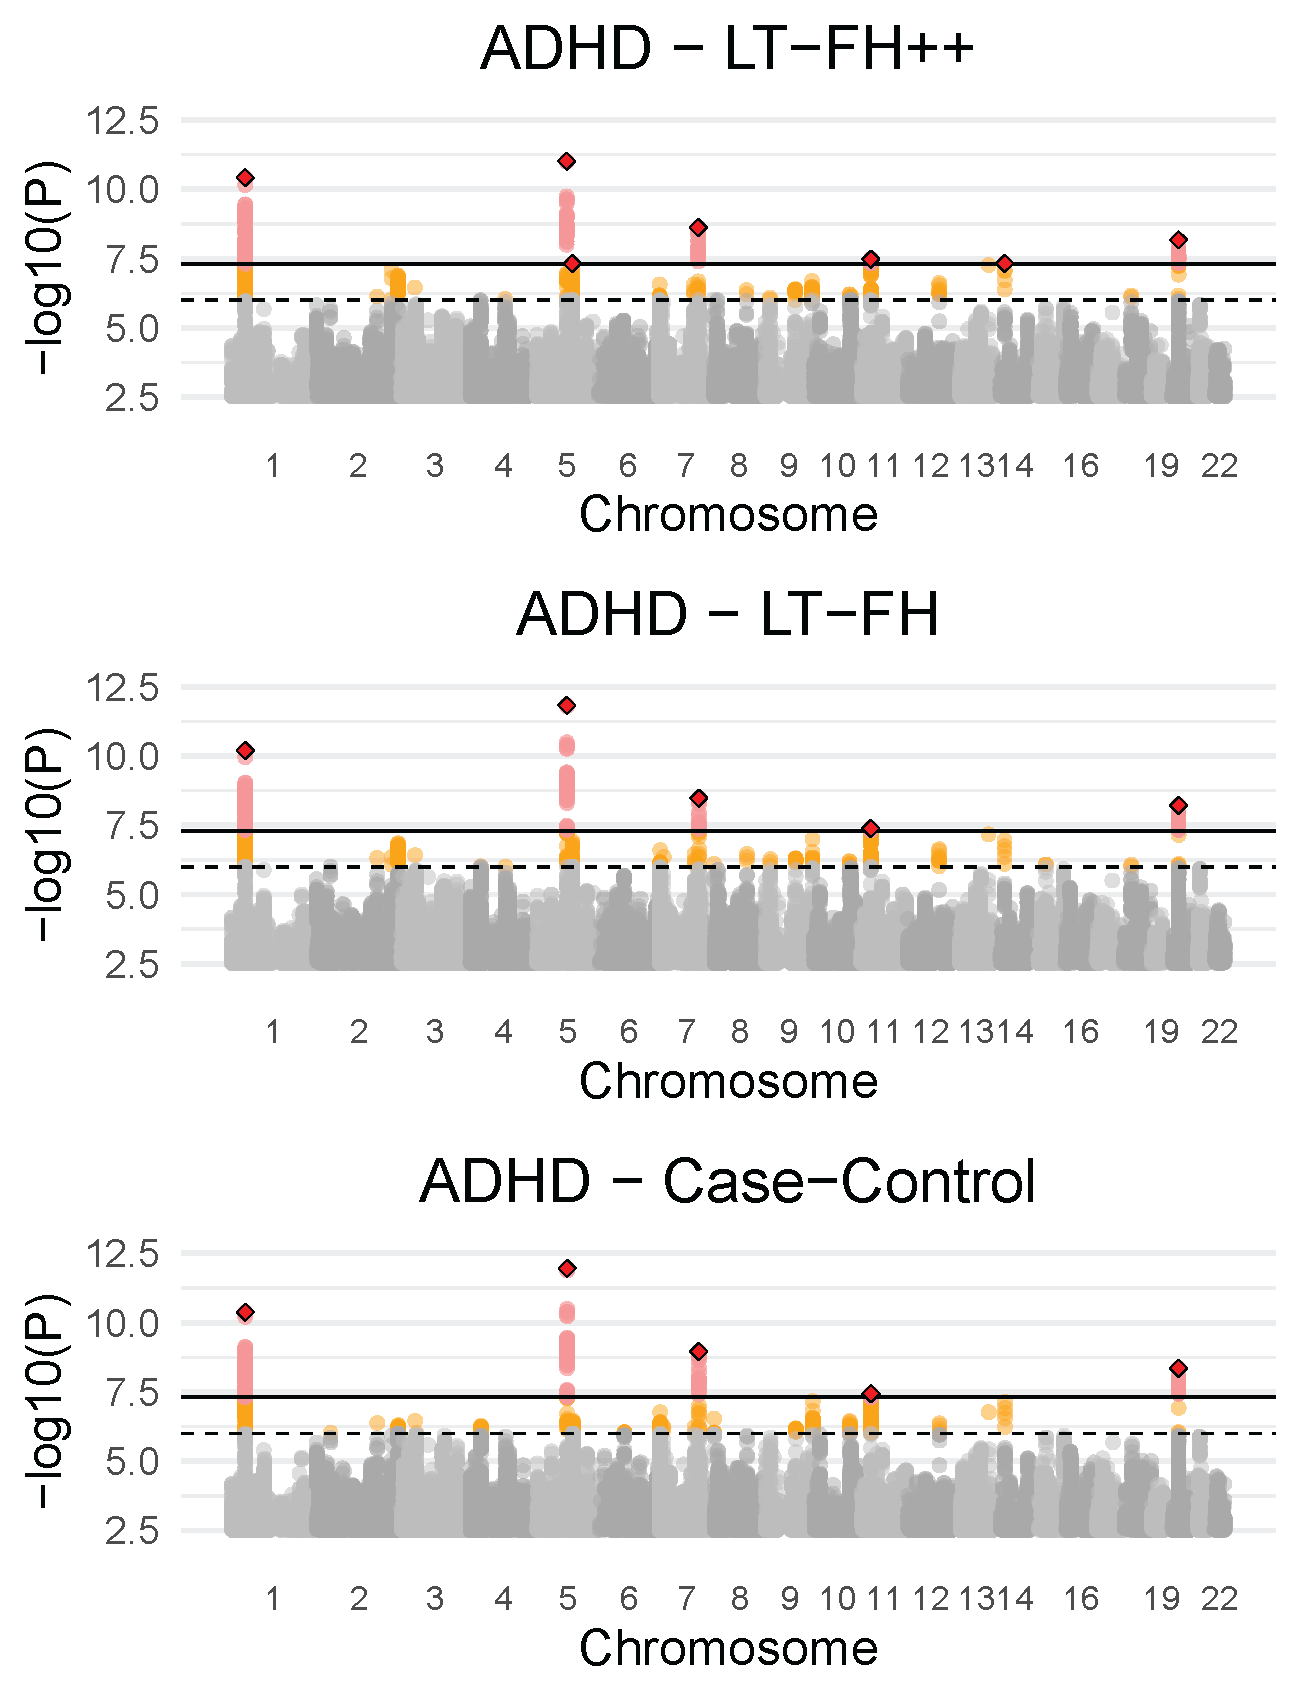
\includegraphics[width=10cm]{results/manhattanPlot_ADHD.png}
\end{wrapfigure}
Through additional simulations we found that one can expect the most \textit{relative} power gain with LT-FH++ over LT-FH if the in-sample prevalence is high in either family members or the index persons. This is due to the fact that LT-FH++ is best able to utilise information for cases, since the CIPs provide a very accurate estimate for the full liability of an individual.